% https://github.com/martinhelso/UiB


\documentclass[UKenglish]{beamer}


\usetheme{UiB}

\usepackage{enumerate}
\usepackage{tabularx}
\usepackage{amsmath,amssymb,amsfonts}

\usepackage[utf8]{inputenx} % For æ, ø, å
\usepackage{csquotes}       % Quotation marks
\usepackage{microtype}      % Improved typography
\usepackage{amssymb}        % Mathematical symbols
\usepackage{mathtools}      % Mathematical symbols
\usepackage[absolute, overlay]{textpos} % Arbitrary placement
\setlength{\TPHorizModule}{\paperwidth} % Textpos units
\setlength{\TPVertModule}{\paperheight} % Textpos units
\usepackage{tikz}
\usetikzlibrary{overlay-beamer-styles}  % Overlay effects for TikZ

\newcommand\numberthis{\addtocounter{equation}{1}\tag{\theequation}}

\author{\small Department of CSE \\ IIT Kharagpur | NITK Surathkal }
\title{Container-based Service State Management in
Cloud Computing}

\subtitle{\small Authors \\ \textbf{Shubha Brata Nath, Sourav Kanti Addya, Sandip Chakraborty and Soumya K Ghosh} }


\begin{document}



% Use
%
%     \begin{frame}[allowframebreaks]{Title}
%
% if the TOC does not fit one frame.
\begin{frame}{Table of contents}
    \tableofcontents[]
\end{frame}



\section{Introduction}
\SectionPage
\subsection{Problem Statement}
\subsection{Solution}
\begin{frame}{Problem Statement}
\vspace{70pt}
To design an efficient mechanism
such that an idle container can be resumed quickly to prevent
the loss of the application’s quality of service (QoS).
\end{frame}
\begin{frame}{Solution}
    \begin{itemize}
\item We propose an exciting direction to significantly boost up the
consolidation ratio of a data-center environment by effectively
managing the container's states
\item We observe that many cloud based application services are event-triggered, so they remain
inactive unless some external service request comes.
\item  We exploit
the fact that the containers remain in an idle state when the
underlying service is not active, and thus such idle containers
can be checkpointed unless an external service request comes.
\item We have
implemented the system, and the evaluation is performed in
Amazon Elastic Compute Cloud. The experimental results have
shown that the proposed algorithm can manage the containers’
states, ensuring the increase of consolidation ratio.
\end{itemize}
\end{frame}

\section{System Architecture}
\SectionPage
\subsection{Architecture Diagram}
\subsection{Docker Container}

\begin{frame}{System Architecture}
    \begin{figure}[htbp]
\centerline{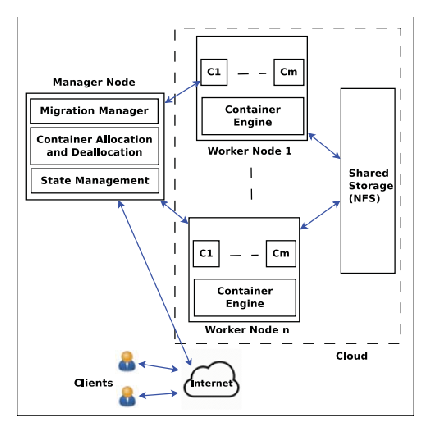
\includegraphics[width=0.5\textwidth]{fig1}}
\caption{System architecture}
\label{fig}
\end{figure}
\end{frame}

\begin{frame}{System Architecture}
     \begin{itemize}
\item Clients: Clients send service request to the manager
node of the cloud data center.
\item Manager Node: The manager node is connected to all
the worker nodes of the cloud data center. The manager
node has a container allocation and deallocation module
to place the services in the cloud data center. This node
does the aggregation of the results. Also, the final result
is sent to the clients. We need to find the status of the
container state (active/idle). This work is performed by
the state management module. 
\item  Cloud Worker Node: The cloud worker node has
container engine (https://docs.docker.com/get-started/
overview/) to run different services as a container.
\item Shared Storage using Network File System: The cloud
worker nodes share a storage to save the state of the
checkpointed containers. This shared storage is designed
using NFS. NFS server is configured in a worker node
that needs to share its directory with other worker nodes.

\end{itemize}
\end{frame}

\begin{frame}{System Architecture}
\vspace{20pt}
    \begin{figure}[htbp]
\centerline{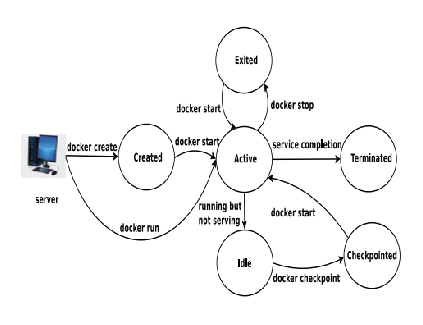
\includegraphics[width=0.5\textwidth]{fig2}}
\caption{Docker Container}
\label{fig}
\end{figure}
\end{frame}


\section{Service State Management of Containerized
Applications}
\SectionPage
\subsection{Average Startup Latency of the Services}
\subsection{Average Response Time of the Services}
\subsection{Constraints}

\begin{frame}{Service State Management of Containerized
Applications}
    Let us consider $C$ containers and $S$ servers present in the
system at a particular time instant. We denote \begin{math} S = \{ S\textsubscript{i} :   i \in (1,...,s) \} \end{math} and \begin{math} C\textsubscript{i} = \{C\textsubscript{j} : j \in (1,...,c)\}\end{math} as sets of cloud
data center servers and containers respectively.

    \begin{alertblock}{Average Startup Latency of the Services}
       \begin{align*} Avg\textsubscript{startup\_latency} =\frac {\sum_{n=1}^{c} Startup\_latency\textsubscript{i}} {c} \end{align*}
    \end{alertblock}

\begin{alertblock}{Average Response Time of the Services}
      \begin{align*} Avg\textsubscript{resp\_time} =\frac {\sum_{n=1}^{c} Resp\_time\textsubscript{i}} {c} ,\end{align*}
    \end{alertblock}
   
\end{frame}

\begin{frame}{Service State Management of Containerized
Applications}
    

    \begin{alertblock}{Constraints}
       \begin{align*} \sum_{j=1}^{TC\textsubscript{i}} C_{j}^{CPU} \times x \textsubscript{i,j} \leq Re_{i}^{CPU} \times y\textsubscript{i} \numberthis \label{eqn} \end{align*}
\begin{align*} \sum_{j=1}^{TC\textsubscript{i}} C_{j}^{RAM} \times x \textsubscript{i,j} \leq Re_{i}^{RAM} \times y\textsubscript{i}\numberthis \label{eqn} \end{align*}
\begin{align*} \sum_{j=1}^{TC\textsubscript{i}} C_{j}^{BW} \times x \textsubscript{i,j} \leq Re_{i}^{BW} \times y\textsubscript{i} \numberthis \label{eqn} \end{align*}
    \end{alertblock}


\end{frame}

\section{Parameters In Amazon EC2 Experiment}
\SectionPage

\begin{frame}{Parameters In Amazon EC2 Experiment}
   \begin{table}[htbp]

\begin{center}
\begin{tabularx}{0.8\textwidth} { 
  | >{\raggedright\arraybackslash}X 
  | >{\centering\arraybackslash}X 
  | >{\raggedleft\arraybackslash}X | }
 \hline
 \textbf{Parameter} & \textbf{Value}  \\
 \hline
 Number of Amazon EC2 virtual
machine instances or worker nodes  & 10    \\
\hline
Processor of a worker node & 2.5 GHz Intel Xeon Family \\ 
\hline 
Number of vCPU in a worker node & 1 \\ 
\hline 
Storage of a worker node & 8 GB \\
\hline 
Operating System used & Ubuntu Server 18.04 LTS \\
\hline
Maximum available RAM of the
worker node & 680 MB \\
\hline
Maximum available RAM of the
manager node & 1780 MB \\
\hline
\end{tabularx}

\end{center}
\end{table}
\end{frame}

\section{Conclusion}
\SectionPage

\begin{frame}{Conclusion}
\begin{itemize}
\item We have performed the container-based service state management to maximize the cloud data center’s consolidation ratio. In our proposed approach, the idle containers need to
be checkpointed to save the hardware resources. However,
after the end of the idle period, the containers need to be
resumed from the last saved state. 
\item The idle containers are
migrated to a new server if the current server does not have
sufficient resources to run it. The problem of state management
of the containers is formulated as an optimization problem that
maximizes the consolidation ratio as the objective function. 
\item The evaluation in Amazon EC2
shows that the proposed algorithm is able to maximize the
consolidation ratio ensuring the state management of the containers. 
\item Thus, the proposed algorithm can efficiently manage
the service state.
\end{itemize}
\end{frame}


\section{References}
\SectionPage

\begin{frame}[allowframebreaks]{References}
    \begin{thebibliography}{}

        

        \setbeamertemplate{bibliography item}[text]

        \bibitem{b1}  E. Casalicchio, “Container orchestration: A survey,” in Systems Modeling: Methodologies and Tools. Springer, 2019, pp. 221–235.
\bibitem{b2} F. Rossi, V. Cardellini, and F. L. Presti, “Elastic deployment of software
containers in geo-distributed computing environments,” in Proc. of IEEE
ISCC’19, 2019.
\bibitem{b3}  K. Suo, Y. Zhao, W. Chen, and J. Rao, “An analysis and empirical
study of container networks,” in proceedings of the IEEE Conference
on Computer Communications. IEEE, 2018, pp. 189–197.
\bibitem{b4}  A. Celesti, D. Mulfari, M. Fazio, M. Villari, and A. Puliafito, “Exploring
container virtualization in iot clouds,” in 2016 IEEE International Conference on Smart Computing (SMARTCOMP). IEEE, 2016, pp.1–6.
\bibitem{b5}  A. Celesti, D. Mulfari, A. Galletta, M. Fazio, L. Carnevale, and
M. Villari, “A study on container virtualization for guarantee quality
of service in cloud-of-things,” Future Generation Computer Systems,
vol. 99, pp. 356–364, 2019.
\bibitem{b6}  I. M. A. Jawarneh, P. Bellavista, L. Foschini, G. Martuscelli, R. Montanari, A. Palopoli, and F. Bosi, “Qos and performance metrics for
container-based virtualization in cloud environments,” in Proceedings
of the 20th International Conference on Distributed Computing and
Networking. ACM, 2019, pp. 178–182.
\bibitem{b7}  W. Li, A. Kanso, and A. Gherbi, “Leveraging linux containers to
achieve high availability for cloud services,” in 2015 IEEE International
Conference on Cloud Engineering. IEEE, 2015, pp. 76–83.

    \end{thebibliography}
\end{frame}

\section{THANK YOU}
\SectionPage

\end{document}